\chapter{Volumen}  % Conceptos relativos a la operativa con volumen

El volumen es un pilar clave en el an\'alisis t\'ecnico de los futuros del S\&P 500 (ES), midiendo la actividad del mercado y revelando la fuerza de los movimientos de precios. Este cap\'itulo explora su definici\'on, comportamiento e interpretaci\'on pr\'actica en un marco temporal de 2 minutos, integrando las perspectivas de Anna Coulling, Miguel \"Angel Ram\'irez y Al Brooks para ofrecer una visi\'on completa y aplicable al trading.

\section{Definici\'on y Rol del Volumen}

El volumen en los futuros del ES, disponible a trav\'es de plataformas como CME Group, representa el \textbf{n\'umero total de contratos negociados} en un per\'iodo (e.g., una vela de 2 minutos o un d\'ia), distinto del \textit{open interest} (contratos abiertos no liquidados). Act\'ua como indicador de \textbf{participaci\'on y liquidez}: un volumen alto refleja alta actividad y facilidad para operar, mientras que un volumen bajo sugiere calma o desinter\'es. Anna Coulling lo considera el ``combustible'' del mercado, Miguel \"Angel Ram\'irez la ``huella'' de los operadores institucionales, y Al Brooks un dato secundario frente a la acci\'on del precio.

\section{Comportamiento e Interpretaci\'on del Volumen}

El volumen var\'ia seg\'un las condiciones del mercado. Permite evaluar la fuerza y validez de los movimientos de precios:

\begin{itemize}
    \item \textbf{Alta actividad}: Se incrementa con \textbf{volatilidad} (e.g., tras noticias econ\'omicas), \textbf{rupturas de niveles t\'ecnicos} (soportes/resistencias), o en la \textbf{apertura y cierre} de la sesi\'on. Un volumen alto con precio ascendente indica una tendencia alcista s\'olida (Coulling: validaci\'on institucional; Ram\'irez: intenci\'on profesional), y lo mismo aplica a ca\'idas con volumen elevado (tendencia bajista fuerte).
    \item \textbf{Baja actividad}: Disminuye en \textbf{mercados laterales}, \textbf{sin eventos relevantes} o \textbf{festividades}. Si el precio se mueve con volumen bajo, sugiere debilidad o posible reversi\'on (divergencia como trampa, Coulling y Ram\'irez).
    \item \textbf{Equilibrio}: Raro, pero en \textbf{tendencias sostenidas} puede estabilizarse, reflejando oferta y demanda equilibradas. En retrocesos dentro de tendencias alcistas, un volumen menor confirma continuidad.
\end{itemize}

\section{Aplicaci\'on Pr\'actica en 2 Minutos}

El volumen es esencial en operativa de corto plazo (2 minutos), permitiendo validar movimientos y detectar trampas. Aqu\'i se integran los enfoques de los autores con su aplicaci\'on:
\subsection{Rupturas y Volumen de Intenci\'on de Verdad}

En marcos de 2 minutos, el \textbf{volumen act\'ua como validaci\'on inmediata} de la intenci\'on profesional al romper zonas clave. El siguiente caso lo ilustra con claridad:

\begin{itemize}
    \sloppy
    \item En la zona resaltada del gr\'afico, el precio rompe al alza una \textbf{resistencia relevante ubicada en los 5750 puntos}, con una \textbf{vela vertical de gran rango} y un \textbf{aumento abrupto del volumen}, superior a los 2000 contratos. Esta acci\'on sugiere \textbf{intenci\'on verdadera}, en t\'erminos de Ram\'irez.
    \item La ruptura se origina tras superar tambi\'en una \textbf{zona previa de resistencia estructural en torno a los 5700 puntos}, lo que refuerza inicialmente la lectura alcista.
    \item Sin embargo, la continuidad falla: el precio no sostiene el avance y regresa con velocidad al rango anterior, cayendo por debajo de los \textbf{5700 puntos}. La \textbf{vela bajista posterior se produce con volumen decreciente}, lo que denota falta de continuidad institucional y posibles ventas encubiertas.
    \item Para Ram\'irez, esto configura una \textbf{trampa profesional}, donde se induce la entrada compradora para facilitar la \textbf{distribuci\'on en resistencia}. Coulling destacar\'ia la \textbf{divergencia entre precio y volumen}, y Brooks no asumir\'ia la ruptura como v\'alida sin una segunda vela de confirmaci\'on posterior al quiebre.
\end{itemize}

\noindent
Este ejemplo enfatiza que el volumen no solo debe confirmar la ruptura inicial, sino tambi\'en \textbf{sostener la acci\'on posterior}. La falta de continuidad o el retroceso r\'apido con volumen bajo por debajo de los \textbf{niveles clave (5750 y 5700)} son \textbf{se\~nales de alerta} para el operador consciente de la acci\'on profesional oculta.

\begin{figure}[!htbp]
  \centering
  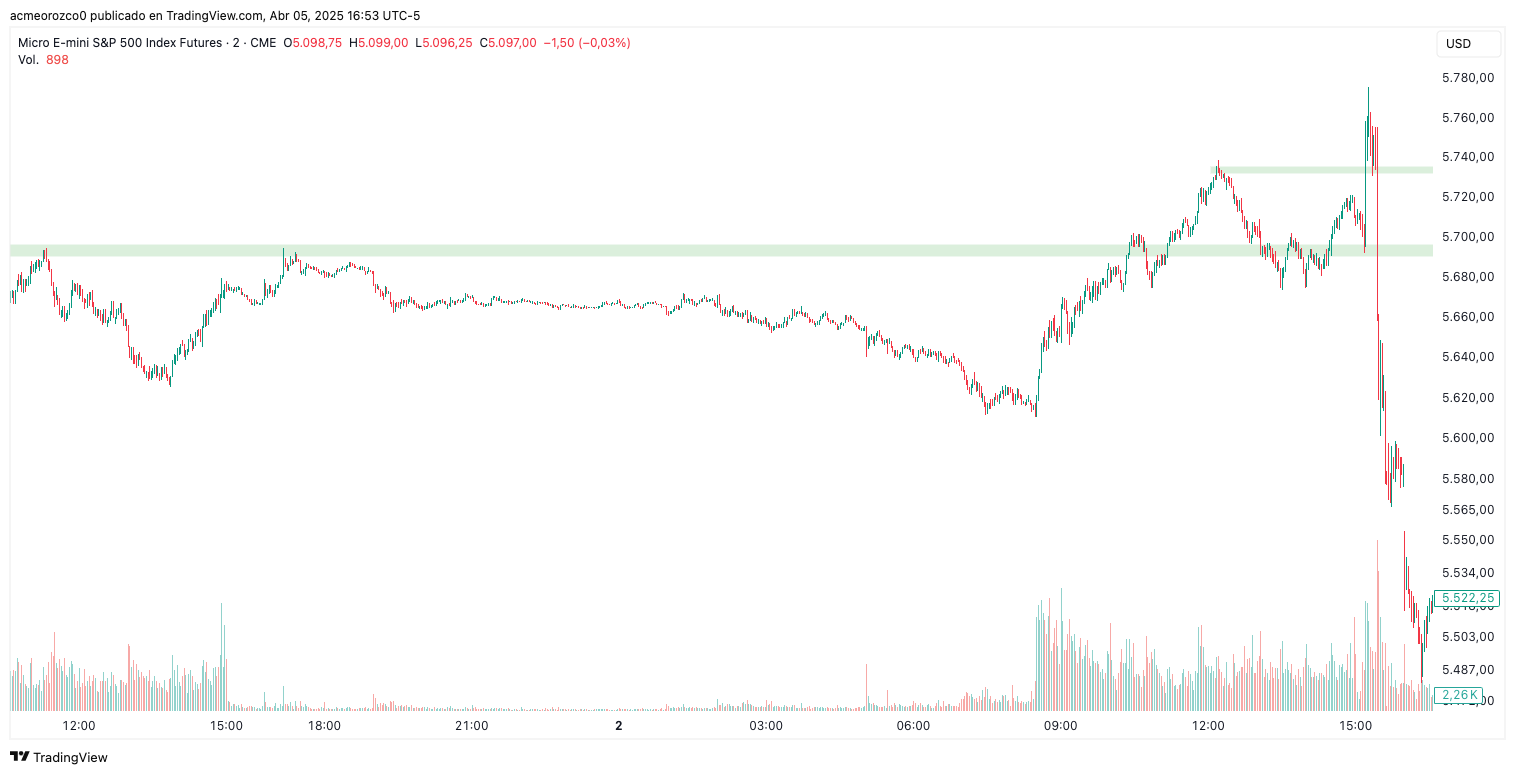
\includegraphics[width=11cm]{images/ruptura_volumen_intencion_2min.png}
  \caption{Ejemplo de ruptura con volumen de intenci\'on en marco de 2 minutos (MES-0625)}
  \label{fig:ruptura_volumen_intencion_2min}
\end{figure}

\vspace{1em}
\noindent
En la figura \ref{fig:ruptura_volumen_intencion_2min} se ilustra una aplicaci\'on pr\'actica del volumen como herramienta de validaci\'on de rupturas en marcos de \textbf{2 minutos}, integrando los enfoques de Ram\'irez, Coulling y Brooks. 

\begin{itemize}
  \sloppy
  \item En la zona destacada, el precio rompe a la baja dos \textbf{zonas de soporte relevantes}, en torno a los \textbf{5720} y \textbf{5700 puntos}, tras una fase de reacumulaci\'on que funcion\'o como \textbf{testeo fallido}. La ruptura se produce con una \textbf{vela de gran rango bajista} y un \textbf{volumen abruptamente creciente}, que alcanza m\'as de 2200 contratos, lo que, seg\'un Ram\'irez, confirma \textbf{intenci\'on profesional vendedora}.
  \item El precio no retrocede tras la ruptura, sino que \textbf{contin\'ua descendiendo} en las siguientes velas con volumen sostenido, lo cual refuerza la validez de la se\~nal. Para Coulling, esta acci\'on representa una \textbf{confirmaci\'on cuantitativa} mediante el volumen: ruptura con desplazamiento y persistencia.
  \item El escenario no presenta indicios de trampa: \textbf{no hay retroceso r\'apido ni rechazo con volumen decreciente}. Esto descarta la posibilidad de una dilataci\'on profesional o falsa ruptura.
  \item Desde la perspectiva de Al Brooks, la acci\'on posterior es clave: el \textbf{cierre fuerte por debajo del soporte}, seguido de otra vela de continuidad bajista, representa la estructura ideal para validar la ruptura sin depender exclusivamente del volumen.
\end{itemize}

\noindent
Este ejemplo refleja la convergencia de los tres autores en la lectura del volumen como confirmaci\'on de la ruptura, aunque cada uno aporta matices: Ram\'irez enfatiza la \textbf{intenci\'on profesional oculta y el contexto de volumen}; Coulling, la \textbf{validaci\'on objetiva de la actividad institucional}; y Brooks, la \textbf{estructura secuencial de velas} para confirmar entradas. Esta integraci\'on permite tomar decisiones m\'as robustas en marcos operativos acelerados como el de 2 minutos.

\begin{figure}[!htbp]
  \centering
  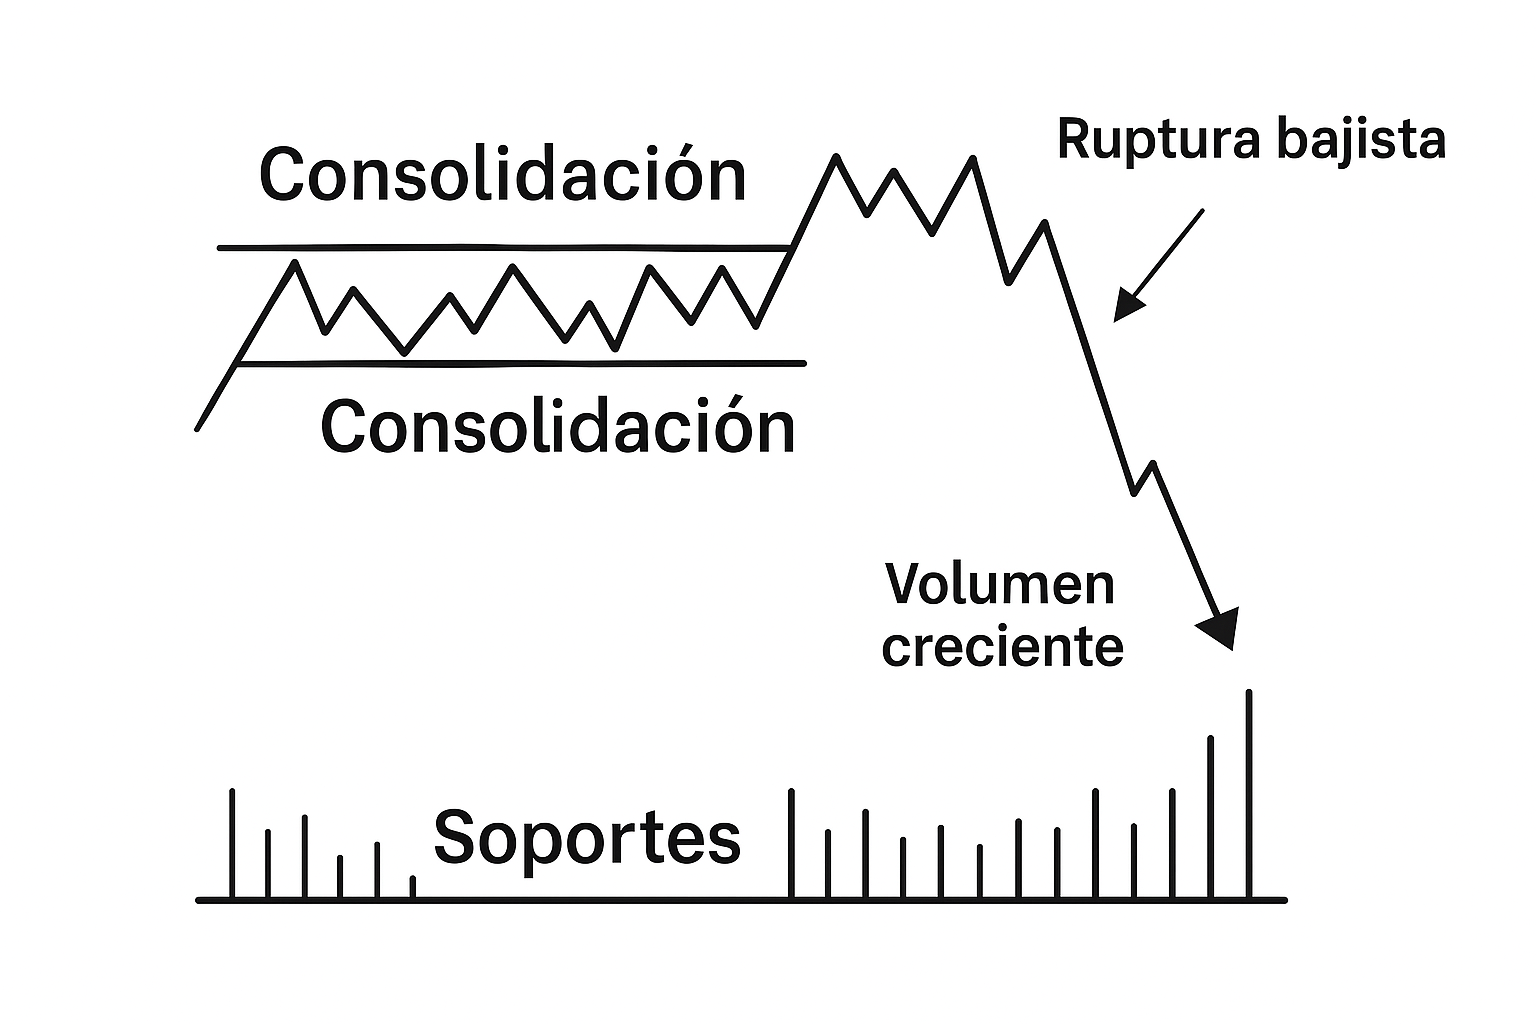
\includegraphics[width=11cm]{images/esquema_ruptura_volumen.png}
  \caption{Ejemplo did\'actico de ruptura con volumen de intenci\'on en marco de 2 minutos (MES-0625)}
  \label{fig:esquema_ruptura_volumen}
\end{figure}

\vspace{1em}
\noindent
La figura \ref{fig:esquema_ruptura_volumen} presenta una \textbf{representaci\'on esquem\'atica} del concepto de \textbf{ruptura con volumen de intenci\'on verdadera}, tal como lo abordan Ram\'irez, Coulling y Brooks en marcos de \textbf{2 minutos}.

\begin{itemize}
  \sloppy  
  \item El gr\'afico muestra una \textbf{zona lateral de consolidaci\'on}, seguida de una \textbf{vela de ruptura bajista de amplio rango}, que irrumpe con fuerza por debajo de un \textbf{soporte clave} previamente testado.    
    \item La ruptura est\'a acompa\~nada por un \textbf{volumen abruptamente creciente}, visible en las barras inferiores. Este comportamiento ilustra lo que Ram\'irez denomina \textbf{intenci\'on institucional}, donde los profesionales ejecutan la ruptura para generar desequilibrio.    
    \item Las velas subsiguientes contin\'uan el desplazamiento a la baja con volumen sostenido, lo que representa una \textbf{validaci\'on t\'ecnica}, seg\'un Coulling, por persistencia en la actividad institucional.
    \item Brooks interpretar\'ia la se\~nal como v\'alida s\'olo si, tras la vela de ruptura, aparece una \textbf{segunda vela bajista} que confirma el movimiento. El esquema refleja esta condici\'on con claridad.
    \item La ausencia de retroceso inmediato o de rechazo con volumen bajo descarta la posibilidad de una \textbf{falsa ruptura o dilataci\'on}.
\end{itemize}

\noindent
Este esquema cumple una funci\'on \textbf{pedag\'ogica} al permitir contrastar una ruptura genuina con otras figuras como las trampas o dilataciones. La convergencia del volumen, el contexto y la continuidad del precio permite una lectura profesional m\'as precisa, alineada con los criterios t\'ecnicos y conductuales propuestos por los autores analizados.


\subsection{Enfoques y Estrategias}
\begin{itemize}
    \item \textbf{Anna Coulling (VPA)}: Usa el volumen para confirmar tendencias y rupturas. Una divergencia (precio sube, volumen baja) indica agotamiento. En 2 minutos, una vela alcista con volumen creciente cerca de un soporte es una entrada; si el volumen cae tras un rally, sugiere salida.
    \item \textbf{Miguel \'Angel Ram\'irez}: Ve el volumen como huella profesional:
    \begin{itemize}
        \item \textbf{Intenci\'on}: Picos (e.g., 5000 contratos tras noticia) muestran acumulaci\'on o distribuci\'on.
        \item \textbf{Testeo}: Volumen bajo (e.g., 800 contratos) en un soporte prueba demanda; un rebote con volumen creciente confirma entrada.
        \item \textbf{Secado}: Volumen decreciente (e.g., 4000 a 1000 contratos en un rally) indica fin de tendencia, ideal para salir o revertir.
    \end{itemize}
    \item \textbf{Al Brooks}: Descarta el volumen, enfoc\'andose en patrones de velas (e.g., doble techo). En 2 minutos, prioriza la acci\'on del precio sobre datos volum\'etricos.
\end{itemize}


\section{Cap\'itulo 12: Volumen y Precio -- La Siguiente Generaci\'on}

En el \'ultimo cap\'itulo, la autora presenta herramientas y conceptos que representan la evoluci\'on contempor\'anea del an\'alisis de volumen. Estas innovaciones permiten una lectura m\'as rica de la acci\'on institucional en los mercados modernos.

\subsection{Gr\'afico de vela-volumen}

Este tipo de gr\'afico conserva la estructura de la vela japonesa, pero ajusta su \textbf{ancho} en proporci\'on al volumen negociado. Una vela ancha indica alta participaci\'on; una vela estrecha, bajo volumen.

\begin{itemize}
  \item Permite visualizar en una misma figura precio y volumen.
  \item Revela si un movimiento amplio ocurri\'o con escaso apoyo institucional.
  \item Es especialmente \'util en ruptura de rangos o validaci\'on de tendencias.
\end{itemize}

\subsection{Volumen delta}

El \textbf{volumen delta} representa la diferencia entre contratos comprados en el \textit{ask} y vendidos en el \textit{bid}:
\[ \Delta = \text{Volumen en el Ask} - \text{Volumen en el Bid} \]

\begin{itemize}
  \item $\Delta > 0$: dominancia de compradores agresivos.
  \item $\Delta < 0$: presi\'on vendedora dominante.
\end{itemize}

\subsection{Volumen delta acumulado}

Este indicador suma el delta barra a barra para construir una curva acumulativa que refleja:
\begin{itemize}
  \item Tendencias sostenidas de compra o venta.
  \item Divergencias con el precio (precio en alza pero delta bajando).
  \item Confirmaci\'on o invalidaci\'on de rompimientos.
\end{itemize}

\subsection{Conclusi\'on del cap\'itulo}

Coulling concluye que estas herramientas no deben reemplazar al VPA tradicional, sino potenciarlo. Mientras el an\'alisis cl\'asico de volumen y precio proporciona el fundamento estructural, estas nuevas t\'ecnicas a\~naden profundidad operativa y precisi\'on t\'actica.

\section{Cap\'itulo 6: An\'alisis del Precio por Volumen -- El Siguiente Nivel}

Este cap\'itulo ampl\'ia la visi\'on b\'asica del \textit{An\'alisis del Precio por Volumen} (VPA), integrando patrones de velas japonesas, estructuras de volumen y contexto t\'ecnico avanzado. Coulling presenta los conceptos de ``volumen de parada'' y ``volumen m\'aximo'' como herramientas clave para anticipar giros o confirmaciones de tendencia~\cite{Coulling13}.

\subsection{Patrones de Velas Clave}

No se trata de aprender todo el diccionario de velas japonesas, sino de identificar aquellas que, en combinaci\'on con el volumen, brindan se\~nales claras de acumulaci\'on, distribuci\'on, agotamiento o confirmaci\'on. Coulling se enfoca en:
\begin{itemize}
  \item Velas con mecha inferior larga: potencial absorci\'on en m\'inimos.
  \item Velas con mecha superior larga: presi\'on vendedora, posible distribuci\'on.
  \item Cuerpos peque\~nos con volumen an\'omalo: incertidumbre en zonas clave.
\end{itemize}

\subsection{Volumen de parada}

Aparece al final de una tendencia y sugiere que las ``manos fuertes'' est\'an cerrando posiciones. Suele ir acompa\~nado de:
\begin{itemize}
  \item Volumen ultra alto.
  \item Rechazo del precio (mechas largas).
  \item Velas de indecisi\'on o de giro.
\end{itemize}

\subsection{Volumen m\'aximo}

Representa una explosi\'on de participaci\'on que valida un rompimiento:
\begin{itemize}
  \item Si el volumen es alto pero el precio no progresa: trampa.
  \item Si el volumen es alto y el precio cierra cerca del extremo: respaldo institucional.
\end{itemize}

\subsection{Perspectiva de an\'alisis}

El VPA no es una t\'ecnica r\'igida, sino un arte. Lo importante es establecer una narrativa l\'ogica entre lo que hace el precio y el volumen.

\subsection{Complemento de Miguel \'Angel Ram\'irez}

Ram\'irez propone el \textbf{volumen relativo} y tres conceptos operativos~\cite{ramirez18}:
\begin{itemize}
  \item \textbf{Intenci\'on}: ruptura respaldada por volumen significativo.
  \item \textbf{Testeo}: movimiento correctivo con volumen bajo.
  \item \textbf{Secado}: desaparici\'on del volumen contrario.
\end{itemize}

\subsection{S\'intesis metodol\'ogica y Criterio compartido}

Ambos autores coinciden: el volumen debe ser interpretado con el contexto. No importa el volumen aislado, sino su efecto en el precio. El an\'alisis se completa con estructura, contexto y consecuencia.

\section{Conclusi\'on}

El volumen es una herramienta vital para traders del ES, con enfoques complementarios:
\begin{itemize}
    \item Coulling: Confirmaci\'on t\'ecnica v\'ia VPA.
    \item Ram\'irez: Narrativa estrat\'egica profesional.
    \item Brooks: Precio como prioridad.
\end{itemize}

En 2 minutos, combina estos principios: verifica tendencias con volumen (Coulling), detecta intenciones y trampas (Ram\'irez), y ajusta con acci\'on del precio (Brooks). Para operar, analiza el volumen en niveles clave, confirma con patrones o indicadores, y act\'ua solo ante se\~nales claras, optimizando as\'i tus decisiones.

El volumen es un pilar clave en el an\'alisis t\'ecnico de los futuros del S\&P 500 (ES), midiendo la actividad del mercado y revelando la fuerza de los movimientos de precios. Este cap\'itulo explora su definici\'on, comportamiento e interpretaci\'on pr\'actica en un marco temporal de 2 minutos, integrando las perspectivas de Anna Coulling, Miguel \"Angel Ram\'irez y Al Brooks para ofrecer una visi\'on completa y aplicable al trading.

\section{Definici\'on y Rol del Volumen}

El volumen en los futuros del ES, disponible a trav\'es de plataformas como CME Group, representa el \textbf{n\'umero total de contratos negociados} en un per\'iodo (e.g., una vela de 2 minutos o un d\'ia), distinto del \textit{open interest} (contratos abiertos no liquidados). Act\'ua como indicador de \textbf{participaci\'on y liquidez}: un volumen alto refleja alta actividad y facilidad para operar, mientras que un volumen bajo sugiere calma o desinter\'es. Anna Coulling lo considera el ``combustible'' del mercado, Miguel \"Angel Ram\'irez la ``huella'' de los operadores institucionales, y Al Brooks un dato secundario frente a la acci\'on del precio.

\section{Comportamiento e Interpretaci\'on del Volumen}

El volumen var\'ia seg\'un las condiciones del mercado. Permite evaluar la fuerza y validez de los movimientos de precios:

\begin{itemize}
    \item \textbf{Alta actividad}: Se incrementa con \textbf{volatilidad} (e.g., tras noticias econ\'omicas), \textbf{rupturas de niveles t\'ecnicos} (soportes/resistencias), o en la \textbf{apertura y cierre} de la sesi\'on. Un volumen alto con precio ascendente indica una tendencia alcista s\'olida (Coulling: validaci\'on institucional; Ram\'irez: intenci\'on profesional), y lo mismo aplica a ca\'idas con volumen elevado (tendencia bajista fuerte).
    \item \textbf{Baja actividad}: Disminuye en \textbf{mercados laterales}, \textbf{sin eventos relevantes} o \textbf{festividades}. Si el precio se mueve con volumen bajo, sugiere debilidad o posible reversi\'on (divergencia como trampa, Coulling y Ram\'irez).
    \item \textbf{Equilibrio}: Raro, pero en \textbf{tendencias sostenidas} puede estabilizarse, reflejando oferta y demanda equilibradas. En retrocesos dentro de tendencias alcistas, un volumen menor confirma continuidad.
\end{itemize}

Existen diversas clasificaciones de volumen: \textbf{volumen de parada}, \textbf{volumen de cl\'imax}, \textbf{volumen profesional} y \textbf{volumen de prueba}. Cada uno cumple una funci\'on en la narrativa institucional del mercado y puede ser clave para anticipar transiciones entre fases de acumulaci\'on, distribuci\'on o continuaci\'on.

\section{Aplicaci\'on Pr\'actica en 2 Minutos}

El volumen es esencial en operativa de corto plazo (2 minutos), permitiendo validar movimientos y detectar trampas. Aqu\'i se integran los enfoques de los autores con su aplicaci\'on:

\subsection{Rupturas y Volumen de Intenci\'on de Verdad}
Un \textbf{aumento significativo de volumen} al romper un nivel clave confirma su validez. Si el precio se sostiene, indica ``intenci\'on verdadera'' (fuerza direccional); si retrocede r\'apido con volumen bajo, sugiere una trampa. Por ejemplo, tras un dato del CPI, una ruptura alcista en 5020 con volumen creciente (e.g., de 1000 a 3000 contratos) valida una entrada larga; un retroceso inmediato a 5015 con volumen cayendo a 800 contratos se\~nala distribuci\'on profesional (Ram\'irez). Coulling enfatiza la confirmaci\'on del volumen, mientras Brooks confiar\'ia solo en el precio post-ruptura.

Las falsas rupturas se caracterizan por un movimiento brusco fuera de un rango seguido de un r\'apido retroceso. Si la ruptura ocurre con \textbf{volumen bajo}, es una se\~nal de debilidad. Si ocurre con \textbf{volumen alto pero sin continuidad}, puede ser una maniobra de distribuci\'on institucional. La lectura cuidadosa de la relaci\'on entre volumen y cierre de vela permite filtrar estas situaciones.

\subsection{Enfoques y Estrategias}
\begin{itemize}
    \item \textbf{Anna Coulling (VPA)}: Usa el volumen para confirmar tendencias y rupturas. Una divergencia (precio sube, volumen baja) indica agotamiento. En 2 minutos, una vela alcista con volumen creciente cerca de un soporte es una entrada; si el volumen cae tras un rally, sugiere salida.
    \item \textbf{Miguel \'Angel Ram\'irez}: Ve el volumen como huella profesional:
    \begin{itemize}
        \item \textbf{Intenci\'on}: Picos (e.g., 5000 contratos tras noticia) muestran acumulaci\'on o distribuci\'on.
        \item \textbf{Testeo}: Volumen bajo (e.g., 800 contratos) en un soporte prueba demanda; un rebote con volumen creciente confirma entrada.
        \item \textbf{Secado}: Volumen decreciente (e.g., 4000 a 1000 contratos en un rally) indica fin de tendencia, ideal para salir o revertir.
    \end{itemize}
    \item \textbf{Al Brooks}: Descarta el volumen, enfoc\'andose en patrones de velas (e.g., doble techo). En 2 minutos, prioriza la acci\'on del precio sobre datos volum\'etricos.
\end{itemize}

Observar el volumen relativo entre varias velas consecutivas es esencial. Un aumento progresivo de volumen en tres velas alcistas sugiere una tendencia con respaldo; si la tercera vela tiene cuerpo peque\~no y volumen anormalmente alto, puede implicar distribuci\'on oculta. Esta secuencia es particularmente eficaz en marcos de 2 minutos donde los movimientos institucionales se ocultan en peque\~nos desplazamientos.

La interpretaci\'on del volumen debe ajustarse al contexto fundamental. En d\'ias de publicaciones clave (como NFP, CPI, FOMC), el volumen refleja reacciones a la sorpresa macroecon\'omica. Un spike de volumen inmediatamente posterior al anuncio indica reacci\'on institucional. Comparar este volumen con promedios anteriores permite determinar si hubo absorci\'on o reacci\'on emocional de minoristas.

\subsection{Volumen delta acumulado}

Este indicador suma el delta barra a barra para construir una curva acumulativa que refleja:
\begin{itemize}
  \item Tendencias sostenidas de compra o venta.
  \item Divergencias con el precio (precio en alza pero delta bajando).
  \item Confirmaci\'on o invalidaci\'on de rompimientos.
\end{itemize}

Una lectura avanzada del volumen delta permite detectar \textbf{absorci\'on}: cuando el precio intenta subir, pero el delta es negativo, indica que hay m\'as ventas agresivas contrarrestando el avance. Esta divergencia sugiere que el profesional est\'a vendiendo en la subida, anticipando una posible reversi\'on.

\subsection*{Cuadro Comparativo de Enfoques sobre el Volumen}

\begin{table}[H]
\centering
\renewcommand{\arraystretch}{1.5}
\resizebox{\textwidth}{!}{%
\begin{tabular}{|>{\RaggedRight\arraybackslash}p{4cm}|
                >{\RaggedRight\arraybackslash}p{4cm}|
                >{\RaggedRight\arraybackslash}p{4cm}|
                >{\RaggedRight\arraybackslash}p{4cm}|}
\hline
\textbf{Categor\'ia} & \textbf{Anna Coulling (VPA)} & \textbf{Miguel \'Angel Ram\'irez} & \textbf{Al Brooks} \\
\hline
\textbf{Rol del volumen} & ``Combustible'' del mercado. Validaci\'on de movimientos. & Huella del operador institucional. & Dato secundario frente a la acci\'on del precio. \\
\hline
\textbf{Enfoque metodol\'ogico} & Volumen + velas en contexto. & Volumen relativo, intenci\'on, testeo y secado. & Lectura de patrones de velas y microestructuras. \\
\hline
\textbf{Herramientas clave} & Volumen de parada, volumen m\'aximo, vela-volumen. & Volumen relativo, zonas relevantes, estructura profesional. & Doble techo, rompimientos falsos, swing high/low. \\
\hline
\textbf{Marco temporal preferido} & Cualquier marco. \'Enfasis en 5m y 15m. & Intrad\'ia, sobre todo 2m y 5m. & Muy corto plazo: 1m--5m. \\
\hline
\textbf{Aplicaci\'on pr\'actica} & Confirmar entradas o salidas. Detectar agotamientos. & Validar trampas, anticipar zonas de acci\'on profesional. & Lectura visual pura del precio, sin volumen. \\
\hline
\end{tabular}
} % fin de resizebox
\caption{Comparaci\'on operativa entre los enfoques de Coulling, Ram\'irez y Brooks}
\end{table}

\section*{Estrategia Basada en el Volumen según Anna Coulling (VPA)}

La estrategia de Anna Coulling se fundamenta en el \textbf{Análisis del Precio por Volumen (VPA)}, el cual consiste en interpretar los movimientos del precio en conjunto con las variaciones del volumen para detectar la participación de operadores institucionales. Su aplicación puede resumirse en la siguiente secuencia estratégica:

\begin{enumerate}
    \item \textbf{Identificación del Contexto:}
    \begin{itemize}
        \item Determinar si el mercado se encuentra en fase de \textit{acumulación}, \textit{distribución}, \textit{tendencia} o \textit{lateralidad}.
        \item Confirmar zonas clave de soporte y resistencia, preferiblemente donde ya haya ocurrido participación institucional previa.
    \end{itemize}

    \item \textbf{Observación del Volumen en Relación al Precio:}
    \begin{itemize}
        \item \textbf{Volumen alto + vela amplia} (alcista o bajista): indica \textbf{intención institucional} y posibilidad de ruptura válida.
        \item \textbf{Volumen bajo + movimiento amplio}: puede ser una \textbf{falsa ruptura}.
        \item \textbf{Volumen alto + vela doji o con mechas largas}: indica \textbf{volumen de parada} y posible \textbf{fin de tendencia}.
        \item \textbf{Volumen creciente + velas pequeñas}: sugiere \textbf{absorción} o \textbf{distribución encubierta}.
    \end{itemize}

    \item \textbf{Confirmación con Patrón de Vela:}
    \begin{itemize}
        \item Buscar velas con cuerpos significativos en la dirección esperada (e.g., vela de cambio o vela envolvente).
        \item Evitar entradas basadas en velas sin confirmación de volumen o con estructuras doji solitarias fuera de contexto.
    \end{itemize}

    \item \textbf{Entrada:}
    \begin{itemize}
        \item Entrada un tick por encima o por debajo de la vela de confirmación, dependiendo de la dirección del movimiento.
        \item Idealmente, sobre zonas relevantes, validando con volumen de ruptura.
    \end{itemize}

    \item \textbf{Gestión de la posición:}
    \begin{itemize}
        \item \textbf{Stop Loss}: por debajo del mínimo (en largos) o por encima del máximo (en cortos) de la vela de entrada.
        \item \textbf{Take Profit}: en zonas de resistencia/soporte posteriores o según relación riesgo-beneficio (mínimo 2:1).
        \item \textbf{Salida parcial}: si se detecta volumen de parada o divergencia con el delta acumulado.
    \end{itemize}
\end{enumerate}

\begin{figure}[!htbp]
  \centering
  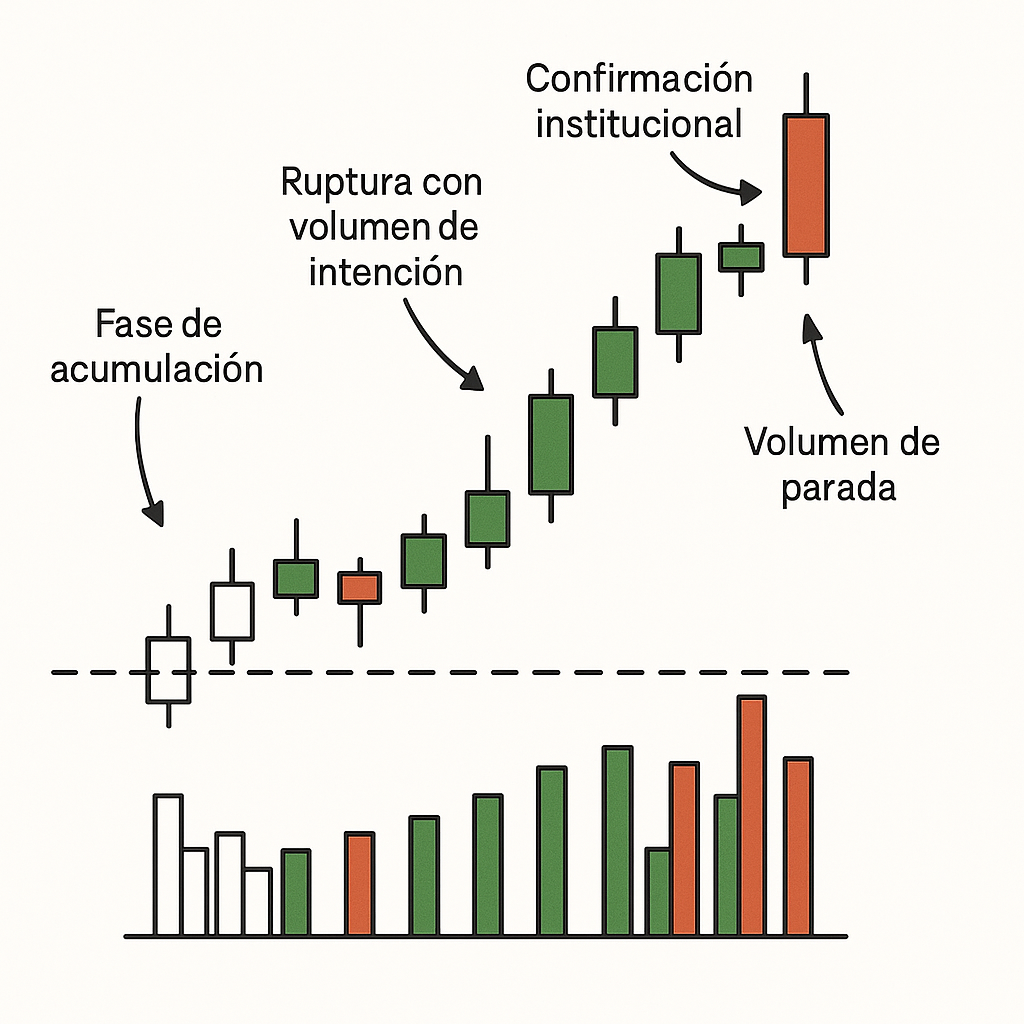
\includegraphics[width=11cm]{images/Vol_Anna_Coulling_Estrategia.png}
  \caption{Ejemplo did\'actico de estrategia basada en volumen seg\'un Anna Coulling (VPA)}
  \label{fig:Vol_Anna_Coulling_Estrategia}
\end{figure}

\vspace{1em}
\noindent
En la figura \ref{fig:Vol_Anna_Coulling_Estrategia} se representa un escenario cl\'asico de aplicaci\'on de la estrategia VPA de Anna Coulling en un marco temporal intrad\'ia (e.g., 5 minutos). El gr\'afico muestra los siguientes eventos clave:

\begin{itemize}
  \item \textbf{Fase de acumulaci\'on}: marcada por velas con cuerpo peque\~no y volumen creciente. Se observa una serie de \textit{velas de incertidumbre} sobre una zona de soporte, lo que sugiere que los operadores profesionales est\'an tomando posiciones sin mover el precio de forma agresiva. 
  \item \textbf{Ruptura con volumen de intenci\'on}: la vela de ruptura (verde) presenta un cuerpo amplio y va acompa\~nada de un \textbf{volumen abruptamente creciente}. Esta combinaci\'on indica que el movimiento cuenta con respaldo institucional y puede tomarse como se\~nal de entrada larga.
  \item \textbf{Confirmaci\'on institucional}: las siguientes velas mantienen la direcci\'on del movimiento con \textbf{volumen sostenido}, reforzando la validez de la ruptura. Coulling considera esta persistencia como prueba de que las ``manos fuertes'' contin\'uan impulsando el precio.
  \item \textbf{Volumen de parada}: tras el rally, aparece una vela con mecha superior larga y volumen ultra alto, sin avance del precio. Esto indica agotamiento de la demanda y posible distribuci\'on. El operador debe evaluar cierre parcial o salida total.
  \item \textbf{Divergencia y correcci\'on}: posteriormente, el volumen comienza a caer mientras el precio sigue subiendo, lo que se interpreta como \textbf{divergencia precio-volumen}. Es una se\~nal t\'ipica de advertencia sobre un posible cambio de tendencia.
\end{itemize}

\noindent
Este ejemplo sintetiza la l\'ogica secuencial de Coulling: \textit{acumulaci\'on silenciosa} $\rightarrow$ \textit{ruptura validada por volumen} $\rightarrow$ \textit{confirmaci\'on por persistencia institucional} $\rightarrow$ \textit{se\~nal de agotamiento por volumen de parada}. El volumen es el protagonista interpretativo en cada fase.

\noindent
Esta estrategia se fortalece especialmente en marcos de \textbf{2 a 15 minutos}, donde el volumen institucional tiende a manifestarse con claridad. Además, puede complementarse con herramientas como el \textit{gráfico vela-volumen}, \textit{volumen delta} y \textit{delta acumulado} para una validación más táctica de la intención profesional.


\section*{Glosario de T\'erminos Clave}

\begin{description}[style=nextline]
  \sloppy
  \item[Volumen] N\'umero total de contratos negociados durante un per\'iodo, o marco de tiempo, espec\'ifico.
  \item[Intenci\'on] Movimiento fuerte en el precio acompa\~nado de volumen significativo que indica presencia institucional.
  \item[Testeo] Movimiento de retroceso con bajo volumen que valida una zona previa como soporte o resistencia.
  \item[Secado] Disminuci\'on notable del volumen que indica retirada del inter\'es profesional y posible cambio de direcci\'on.
  \item[Volumen de parada] Pico abrupto de volumen al final de una tendencia, indicando posible giro.
  \item[Volumen m\'aximo] Alta participaci\'on en una vela que puede confirmar o desmentir un rompimiento t\'ecnico.
  \item[Volumen delta] Diferencia entre compras agresivas (``ask'') y ventas agresivas (``bid'').
  \item[Delta acumulado] Suma progresiva del delta, usada para confirmar la intenci\'on sostenida del mercado.
  \item[Absorci\'on] Situaci\'on en la que el precio se mueve en una direcci\'on, pero el volumen delta indica presi\'on opuesta oculta.
  \item[Distribuci\'on] Venta institucional oculta durante un alza de precio; puede detectarse por divergencias en volumen.
  \item[Acumulaci\'on] Compra institucional disfrazada durante una baja del precio; revelada por patrones y volumen an\'omalo.
\end{description}

